% Generated by Sphinx.
\def\sphinxdocclass{report}
\documentclass[letterpaper,10pt,english]{sphinxmanual}
\usepackage[utf8]{inputenc}
\DeclareUnicodeCharacter{00A0}{\nobreakspace}
\usepackage{cmap}
\usepackage[T1]{fontenc}
\usepackage{babel}
\usepackage{times}
\usepackage[Bjarne]{fncychap}
\usepackage{longtable}
\usepackage{sphinx}
\usepackage{multirow}


\title{CPAT Documentation}
\date{October 10, 2013}
\release{1.2.1}
\author{Liguo Wang, Hyun Jung Park}
\newcommand{\sphinxlogo}{}
\renewcommand{\releasename}{Release}
\makeindex

\makeatletter
\def\PYG@reset{\let\PYG@it=\relax \let\PYG@bf=\relax%
    \let\PYG@ul=\relax \let\PYG@tc=\relax%
    \let\PYG@bc=\relax \let\PYG@ff=\relax}
\def\PYG@tok#1{\csname PYG@tok@#1\endcsname}
\def\PYG@toks#1+{\ifx\relax#1\empty\else%
    \PYG@tok{#1}\expandafter\PYG@toks\fi}
\def\PYG@do#1{\PYG@bc{\PYG@tc{\PYG@ul{%
    \PYG@it{\PYG@bf{\PYG@ff{#1}}}}}}}
\def\PYG#1#2{\PYG@reset\PYG@toks#1+\relax+\PYG@do{#2}}

\expandafter\def\csname PYG@tok@gd\endcsname{\def\PYG@tc##1{\textcolor[rgb]{0.63,0.00,0.00}{##1}}}
\expandafter\def\csname PYG@tok@gu\endcsname{\let\PYG@bf=\textbf\def\PYG@tc##1{\textcolor[rgb]{0.50,0.00,0.50}{##1}}}
\expandafter\def\csname PYG@tok@gt\endcsname{\def\PYG@tc##1{\textcolor[rgb]{0.00,0.27,0.87}{##1}}}
\expandafter\def\csname PYG@tok@gs\endcsname{\let\PYG@bf=\textbf}
\expandafter\def\csname PYG@tok@gr\endcsname{\def\PYG@tc##1{\textcolor[rgb]{1.00,0.00,0.00}{##1}}}
\expandafter\def\csname PYG@tok@cm\endcsname{\let\PYG@it=\textit\def\PYG@tc##1{\textcolor[rgb]{0.25,0.50,0.56}{##1}}}
\expandafter\def\csname PYG@tok@vg\endcsname{\def\PYG@tc##1{\textcolor[rgb]{0.73,0.38,0.84}{##1}}}
\expandafter\def\csname PYG@tok@m\endcsname{\def\PYG@tc##1{\textcolor[rgb]{0.13,0.50,0.31}{##1}}}
\expandafter\def\csname PYG@tok@mh\endcsname{\def\PYG@tc##1{\textcolor[rgb]{0.13,0.50,0.31}{##1}}}
\expandafter\def\csname PYG@tok@cs\endcsname{\def\PYG@tc##1{\textcolor[rgb]{0.25,0.50,0.56}{##1}}\def\PYG@bc##1{\setlength{\fboxsep}{0pt}\colorbox[rgb]{1.00,0.94,0.94}{\strut ##1}}}
\expandafter\def\csname PYG@tok@ge\endcsname{\let\PYG@it=\textit}
\expandafter\def\csname PYG@tok@vc\endcsname{\def\PYG@tc##1{\textcolor[rgb]{0.73,0.38,0.84}{##1}}}
\expandafter\def\csname PYG@tok@il\endcsname{\def\PYG@tc##1{\textcolor[rgb]{0.13,0.50,0.31}{##1}}}
\expandafter\def\csname PYG@tok@go\endcsname{\def\PYG@tc##1{\textcolor[rgb]{0.20,0.20,0.20}{##1}}}
\expandafter\def\csname PYG@tok@cp\endcsname{\def\PYG@tc##1{\textcolor[rgb]{0.00,0.44,0.13}{##1}}}
\expandafter\def\csname PYG@tok@gi\endcsname{\def\PYG@tc##1{\textcolor[rgb]{0.00,0.63,0.00}{##1}}}
\expandafter\def\csname PYG@tok@gh\endcsname{\let\PYG@bf=\textbf\def\PYG@tc##1{\textcolor[rgb]{0.00,0.00,0.50}{##1}}}
\expandafter\def\csname PYG@tok@ni\endcsname{\let\PYG@bf=\textbf\def\PYG@tc##1{\textcolor[rgb]{0.84,0.33,0.22}{##1}}}
\expandafter\def\csname PYG@tok@nl\endcsname{\let\PYG@bf=\textbf\def\PYG@tc##1{\textcolor[rgb]{0.00,0.13,0.44}{##1}}}
\expandafter\def\csname PYG@tok@nn\endcsname{\let\PYG@bf=\textbf\def\PYG@tc##1{\textcolor[rgb]{0.05,0.52,0.71}{##1}}}
\expandafter\def\csname PYG@tok@no\endcsname{\def\PYG@tc##1{\textcolor[rgb]{0.38,0.68,0.84}{##1}}}
\expandafter\def\csname PYG@tok@na\endcsname{\def\PYG@tc##1{\textcolor[rgb]{0.25,0.44,0.63}{##1}}}
\expandafter\def\csname PYG@tok@nb\endcsname{\def\PYG@tc##1{\textcolor[rgb]{0.00,0.44,0.13}{##1}}}
\expandafter\def\csname PYG@tok@nc\endcsname{\let\PYG@bf=\textbf\def\PYG@tc##1{\textcolor[rgb]{0.05,0.52,0.71}{##1}}}
\expandafter\def\csname PYG@tok@nd\endcsname{\let\PYG@bf=\textbf\def\PYG@tc##1{\textcolor[rgb]{0.33,0.33,0.33}{##1}}}
\expandafter\def\csname PYG@tok@ne\endcsname{\def\PYG@tc##1{\textcolor[rgb]{0.00,0.44,0.13}{##1}}}
\expandafter\def\csname PYG@tok@nf\endcsname{\def\PYG@tc##1{\textcolor[rgb]{0.02,0.16,0.49}{##1}}}
\expandafter\def\csname PYG@tok@si\endcsname{\let\PYG@it=\textit\def\PYG@tc##1{\textcolor[rgb]{0.44,0.63,0.82}{##1}}}
\expandafter\def\csname PYG@tok@s2\endcsname{\def\PYG@tc##1{\textcolor[rgb]{0.25,0.44,0.63}{##1}}}
\expandafter\def\csname PYG@tok@vi\endcsname{\def\PYG@tc##1{\textcolor[rgb]{0.73,0.38,0.84}{##1}}}
\expandafter\def\csname PYG@tok@nt\endcsname{\let\PYG@bf=\textbf\def\PYG@tc##1{\textcolor[rgb]{0.02,0.16,0.45}{##1}}}
\expandafter\def\csname PYG@tok@nv\endcsname{\def\PYG@tc##1{\textcolor[rgb]{0.73,0.38,0.84}{##1}}}
\expandafter\def\csname PYG@tok@s1\endcsname{\def\PYG@tc##1{\textcolor[rgb]{0.25,0.44,0.63}{##1}}}
\expandafter\def\csname PYG@tok@gp\endcsname{\let\PYG@bf=\textbf\def\PYG@tc##1{\textcolor[rgb]{0.78,0.36,0.04}{##1}}}
\expandafter\def\csname PYG@tok@sh\endcsname{\def\PYG@tc##1{\textcolor[rgb]{0.25,0.44,0.63}{##1}}}
\expandafter\def\csname PYG@tok@ow\endcsname{\let\PYG@bf=\textbf\def\PYG@tc##1{\textcolor[rgb]{0.00,0.44,0.13}{##1}}}
\expandafter\def\csname PYG@tok@sx\endcsname{\def\PYG@tc##1{\textcolor[rgb]{0.78,0.36,0.04}{##1}}}
\expandafter\def\csname PYG@tok@bp\endcsname{\def\PYG@tc##1{\textcolor[rgb]{0.00,0.44,0.13}{##1}}}
\expandafter\def\csname PYG@tok@c1\endcsname{\let\PYG@it=\textit\def\PYG@tc##1{\textcolor[rgb]{0.25,0.50,0.56}{##1}}}
\expandafter\def\csname PYG@tok@kc\endcsname{\let\PYG@bf=\textbf\def\PYG@tc##1{\textcolor[rgb]{0.00,0.44,0.13}{##1}}}
\expandafter\def\csname PYG@tok@c\endcsname{\let\PYG@it=\textit\def\PYG@tc##1{\textcolor[rgb]{0.25,0.50,0.56}{##1}}}
\expandafter\def\csname PYG@tok@mf\endcsname{\def\PYG@tc##1{\textcolor[rgb]{0.13,0.50,0.31}{##1}}}
\expandafter\def\csname PYG@tok@err\endcsname{\def\PYG@bc##1{\setlength{\fboxsep}{0pt}\fcolorbox[rgb]{1.00,0.00,0.00}{1,1,1}{\strut ##1}}}
\expandafter\def\csname PYG@tok@kd\endcsname{\let\PYG@bf=\textbf\def\PYG@tc##1{\textcolor[rgb]{0.00,0.44,0.13}{##1}}}
\expandafter\def\csname PYG@tok@ss\endcsname{\def\PYG@tc##1{\textcolor[rgb]{0.32,0.47,0.09}{##1}}}
\expandafter\def\csname PYG@tok@sr\endcsname{\def\PYG@tc##1{\textcolor[rgb]{0.14,0.33,0.53}{##1}}}
\expandafter\def\csname PYG@tok@mo\endcsname{\def\PYG@tc##1{\textcolor[rgb]{0.13,0.50,0.31}{##1}}}
\expandafter\def\csname PYG@tok@mi\endcsname{\def\PYG@tc##1{\textcolor[rgb]{0.13,0.50,0.31}{##1}}}
\expandafter\def\csname PYG@tok@kn\endcsname{\let\PYG@bf=\textbf\def\PYG@tc##1{\textcolor[rgb]{0.00,0.44,0.13}{##1}}}
\expandafter\def\csname PYG@tok@o\endcsname{\def\PYG@tc##1{\textcolor[rgb]{0.40,0.40,0.40}{##1}}}
\expandafter\def\csname PYG@tok@kr\endcsname{\let\PYG@bf=\textbf\def\PYG@tc##1{\textcolor[rgb]{0.00,0.44,0.13}{##1}}}
\expandafter\def\csname PYG@tok@s\endcsname{\def\PYG@tc##1{\textcolor[rgb]{0.25,0.44,0.63}{##1}}}
\expandafter\def\csname PYG@tok@kp\endcsname{\def\PYG@tc##1{\textcolor[rgb]{0.00,0.44,0.13}{##1}}}
\expandafter\def\csname PYG@tok@w\endcsname{\def\PYG@tc##1{\textcolor[rgb]{0.73,0.73,0.73}{##1}}}
\expandafter\def\csname PYG@tok@kt\endcsname{\def\PYG@tc##1{\textcolor[rgb]{0.56,0.13,0.00}{##1}}}
\expandafter\def\csname PYG@tok@sc\endcsname{\def\PYG@tc##1{\textcolor[rgb]{0.25,0.44,0.63}{##1}}}
\expandafter\def\csname PYG@tok@sb\endcsname{\def\PYG@tc##1{\textcolor[rgb]{0.25,0.44,0.63}{##1}}}
\expandafter\def\csname PYG@tok@k\endcsname{\let\PYG@bf=\textbf\def\PYG@tc##1{\textcolor[rgb]{0.00,0.44,0.13}{##1}}}
\expandafter\def\csname PYG@tok@se\endcsname{\let\PYG@bf=\textbf\def\PYG@tc##1{\textcolor[rgb]{0.25,0.44,0.63}{##1}}}
\expandafter\def\csname PYG@tok@sd\endcsname{\let\PYG@it=\textit\def\PYG@tc##1{\textcolor[rgb]{0.25,0.44,0.63}{##1}}}

\def\PYGZbs{\char`\\}
\def\PYGZus{\char`\_}
\def\PYGZob{\char`\{}
\def\PYGZcb{\char`\}}
\def\PYGZca{\char`\^}
\def\PYGZam{\char`\&}
\def\PYGZlt{\char`\<}
\def\PYGZgt{\char`\>}
\def\PYGZsh{\char`\#}
\def\PYGZpc{\char`\%}
\def\PYGZdl{\char`\$}
\def\PYGZhy{\char`\-}
\def\PYGZsq{\char`\'}
\def\PYGZdq{\char`\"}
\def\PYGZti{\char`\~}
% for compatibility with earlier versions
\def\PYGZat{@}
\def\PYGZlb{[}
\def\PYGZrb{]}
\makeatother

\begin{document}

\maketitle
\tableofcontents
\phantomsection\label{index::doc}
\scalebox{0.500000}{
\includegraphics{cpat.png}}



CPAT v1.2.1
\begin{enumerate}
\item {} 
Support compressed input file ({\color{red}\bfseries{}*}.gz or {\color{red}\bfseries{}*}.bz2)

\item {} 
Support url as input. url should be link (pointing to data repository) starts with \href{http://}{http://}, \href{https://}{https://} or \href{ftp://}{ftp://} .

\end{enumerate}

CPAT v1.2

Conservation score was obsolete. Because it depends on the alignment, relatively slow in
calculation and more importantly very little power is gained by using this feature. We
use hexamer usage bias as the 4th feature:
\begin{enumerate}
\item {} 
ORF (Open Reading Frame) size

\item {} 
ORF coverage (ratio of ORF size to transcript size)

\item {} 
Fickett TESTCODE statistic

\item {} 
Hexamer usage bias

\end{enumerate}

CPAT v1.1:

This is the only version using conservation score (phastCon) as one prediction feature. 4 features used for prediction:
\begin{enumerate}
\item {} 
ORF (Open Reading Frame) size

\item {} 
ORF coverage (ratio of ORF size to transcript size)

\item {} 
Fickett TESTCODE statistic

\item {} 
PhastCon conservation score

\end{enumerate}


\chapter{Introduction}
\label{index:introduction}\label{index:release-history}
Using RNA-seq, tens of thousands of novel transcripts and isoforms have been identified (Djebali, et al  Nature, 2012
, Carbili et al, Gene \& Development, 2011)
The discovery of these hidden transcriptome rejuvenate the need of distinguishing coding
and noncoding RNA. However, Most previous coding potential prediction methods heavily rely
on alignment, either pairwise alignment to search for protein evidence or multiple alignments
to calculate phylogenetic conservation score (such as \href{http://cpc.cbi.pku.edu.cn/}{CPC} , \href{http://compbio.mit.edu/PhyloCSF}{PhyloCSF} and \href{http://wash.github.com/rnacode/}{RNACode} ). This is because most previously identified transcripts
including protein coding RNA and short, housekeeping or regulatory RNAs such as snRNAs,
snoRNA and tRNA are highly conserved. While still very useful, these approaches have several
limitations:
\begin{itemize}
\item {} 
Most lncRNAs are less conserved and tend to be lineage specific which greatly limited the discrimination power of alignment-based methods. For example, of 550 lncRNA detected from zebrafish, only 29 of them had detectable sequence similarity with putative mammalian orthologs (Ulitsky  et al, Cell, 2011).

\item {} 
A significant fraction of protein coding genes may have an alternatively processed isoform or one transcribed from an alternative promoter, these part of ncRNA cannot be correctly classified through homologous search because they would have significant match to protein coding genes.

\item {} 
Alignment based method is extremely slow. For example, \href{http://www.ncbi.nlm.nih.gov/pubmed/17631615}{CPC} takes 6050 CPU minutes (\textgreater{} 4 days) to evaluate 14,000 lncRNA transcripts.

\item {} 
Reliability depends on alignment quality. Most multi-alignment tools use heuristic search and do not guarantee to give optimal alignments.

\end{itemize}

CPAT overcomes the above problems by using logistic regression model based on 4 pure sequence
linguistic features. 1) ORF size, 2) ORF coverage,
3) \href{http://nar.oxfordjournals.org/content/10/17/5303.abstract}{Fickett TESTCODE} and 4)
\href{http://nar.oxfordjournals.org/content/20/24/6441.abstract}{Hexamer usage bais}. Linguistic
feature based method does not require other genomes or protein databases to perform alignment
and is more robust. Because it is alignment free, it runs much faster and also easier to use.
For example,  CPAT takes several minutes to evaluate the above 14,000 lncRNAs. More importantly,
compared with alignment-based approaches, it performs better with improved sensitivity and
specificity (0.966 tested on human gene annotation).

Combinatorial effects of 3 major features. 10,000 coding genes (red dots) and 10,000 noncoding genes (blue dots) are clearly separated into two clusters. (below figure)
\begin{figure}[htbp]
\centering

\scalebox{1.000000}{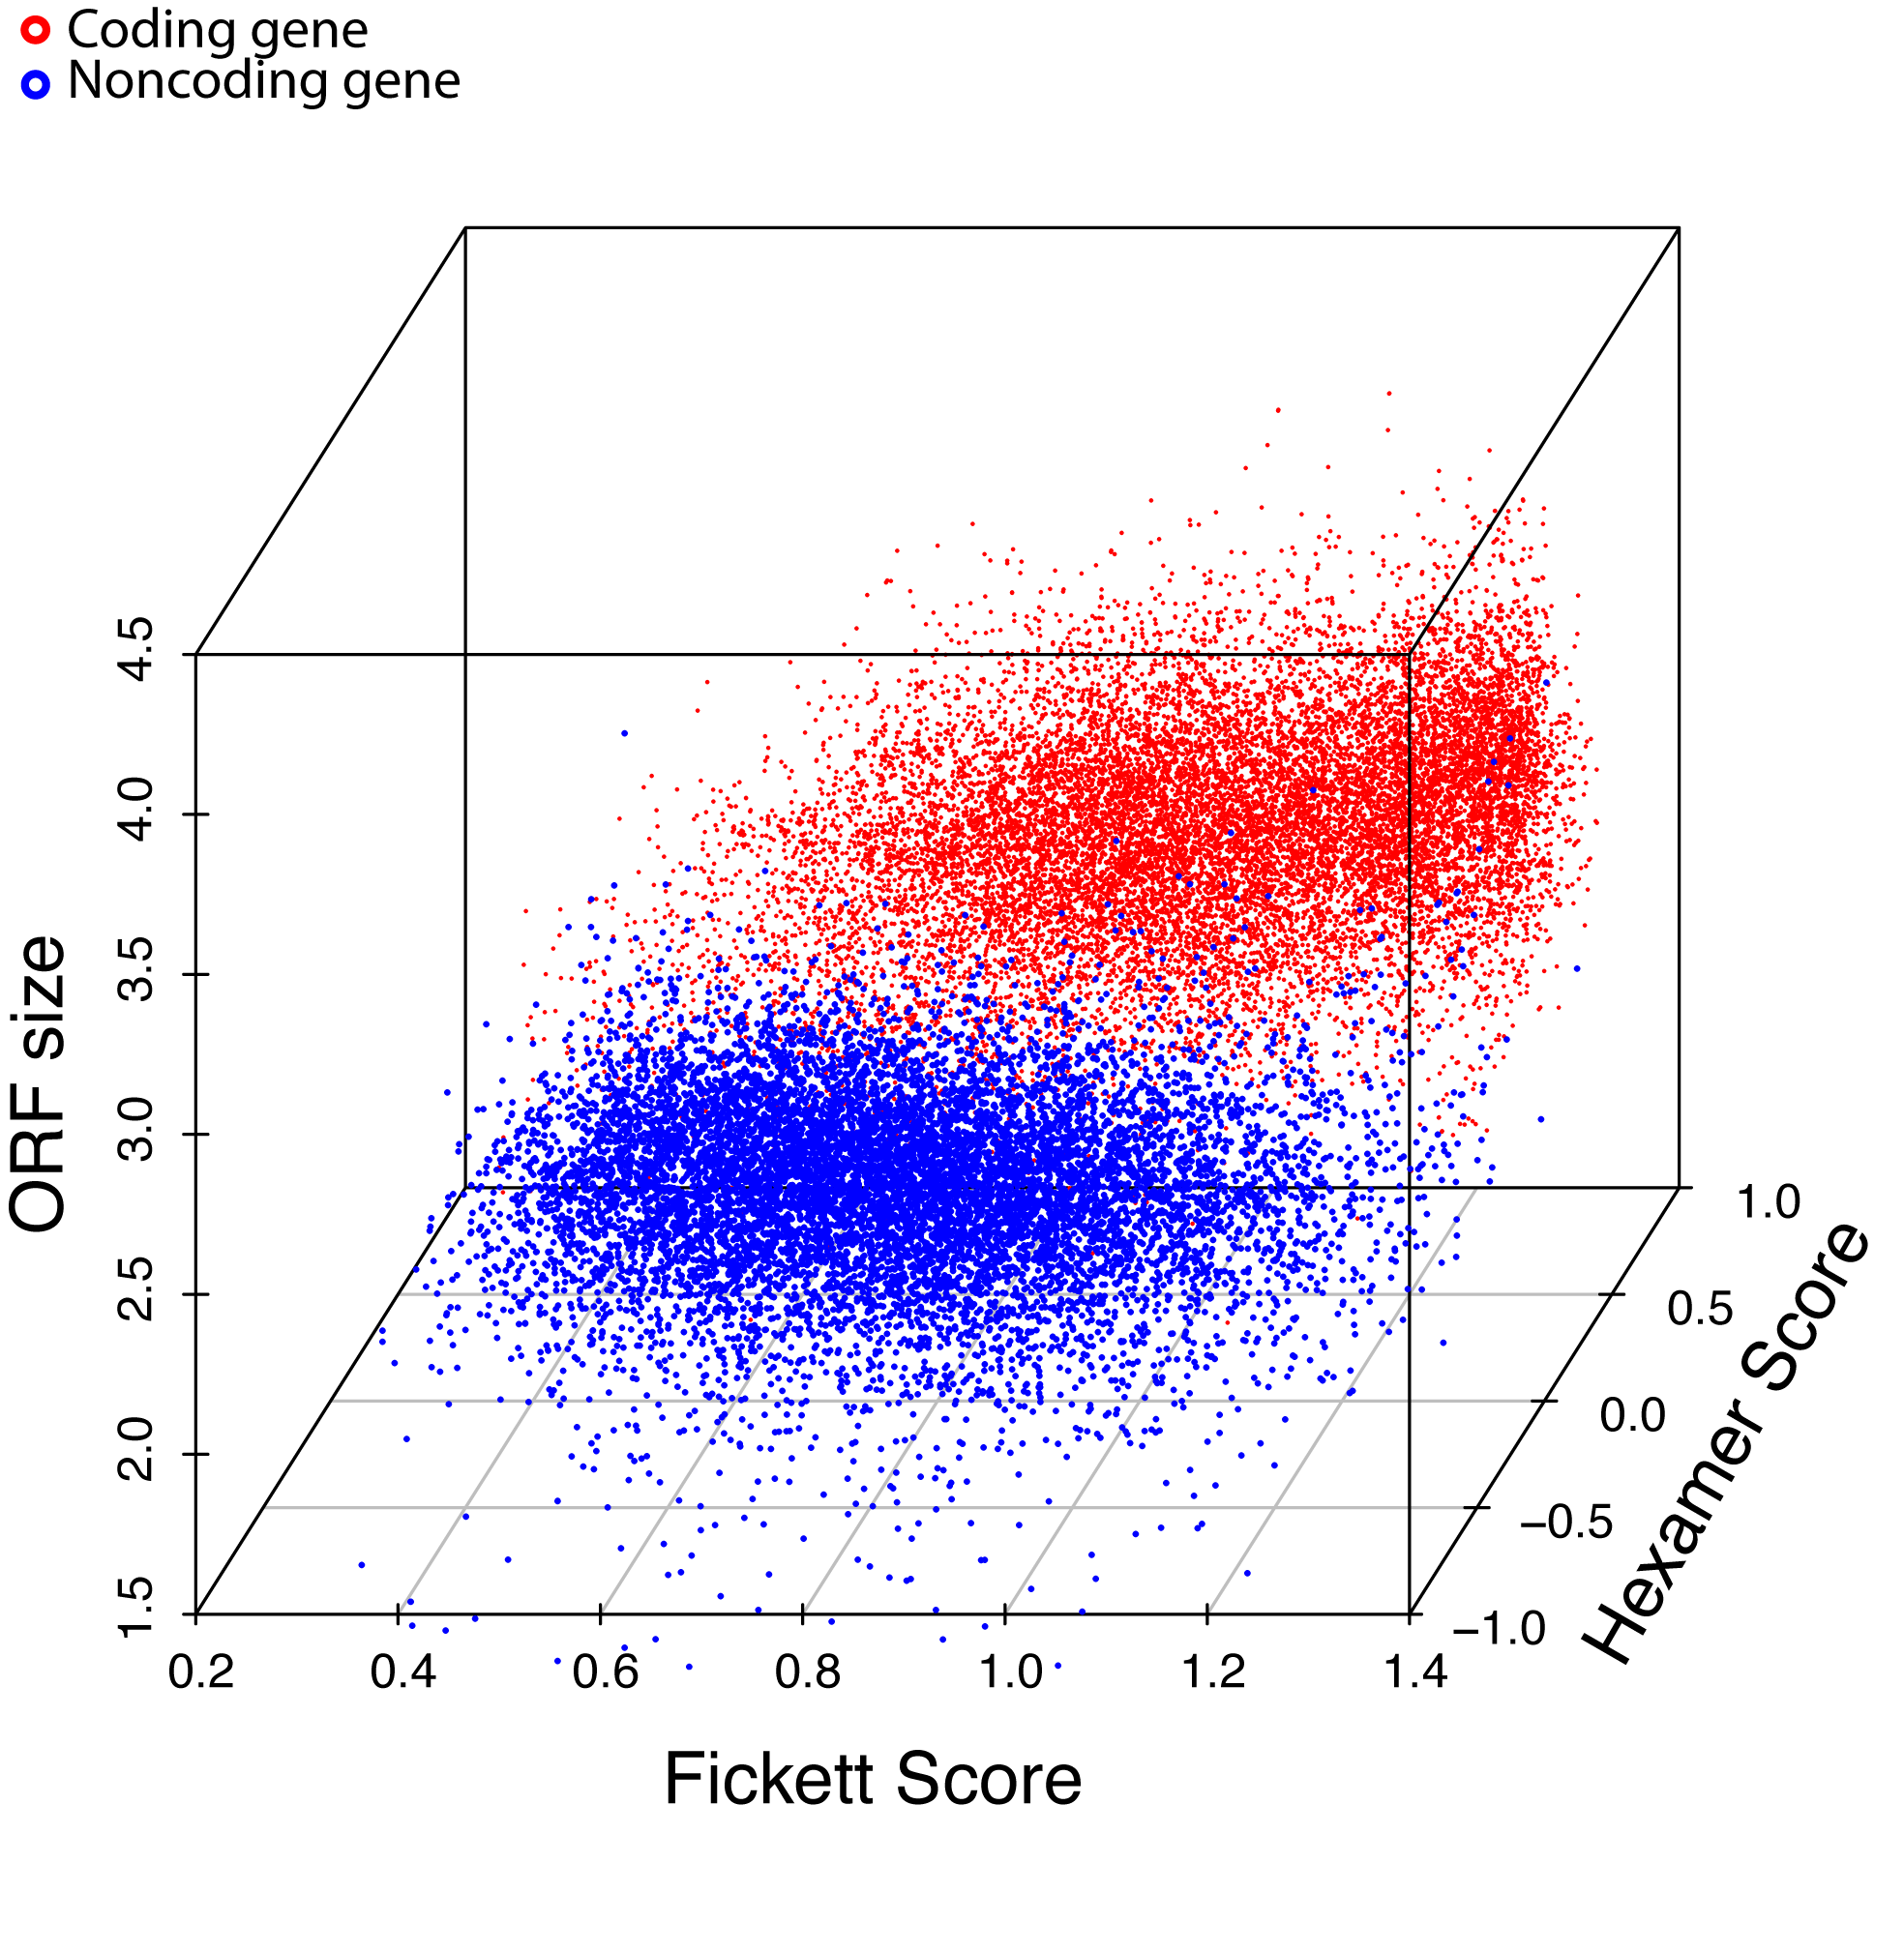
\includegraphics{Figure_1A_features_3D.png}}
\end{figure}


\chapter{Run CPAT online}
\label{index:run-cpat-online}
\href{http://lilab.research.bcm.edu/cpat/}{http://lilab.research.bcm.edu/cpat/}
\begin{itemize}
\item {} 
This web server only supports Human (hg19), Mouse (mm10), Fly (dm3) and Zebrafish (Zv9).

\item {} 
When input file is BED format, the reference genome is required and the assembly version is important. For example, user cannot upload hg18 based BED file to this server, as we only support hg19.

\item {} 
When the input file is FASTA sequence file, the reference genome is NOT required. Because all features can be calculated from the FASTA sequence directly.

\end{itemize}


\section{Step1}
\label{index:step1}
Upload data to CPAT server. There are 3 different ways that user can upload their data:
\begin{itemize}
\item {} 
Upload BED or FASTA format files from local disk. Files can be regular or compressed ({\color{red}\bfseries{}*}.gz, {\color{red}\bfseries{}*}.Z. {\color{red}\bfseries{}*}.z, {\color{red}\bfseries{}*}.bz, {\color{red}\bfseries{}*}.bz2, {\color{red}\bfseries{}*}.bzip2).

\item {} 
For small dataset, user can copy and paste data (in BED or FASTA format) directly to the text area.

\item {} 
For extremely larger dataset, user can save data in web server (http, https or ftp) first, then paste the data url to CPAT.

\end{itemize}


\section{Step2}
\label{index:step2}
Select Select Species assembly


\section{Step3}
\label{index:step3}
Click Submit button


\chapter{Download}
\label{index:download}
\href{https://sourceforge.net/projects/rna-cpat/files/CPAT-1.2.1.tar.gz/download}{CPAT}

prebuilt \href{https://sourceforge.net/projects/rna-cpat/files/prebuilt\_models.zip/download}{logit model and hexamer table} for Human, Mouse, Fly and Zebrafish


\chapter{Installation}
\label{index:installation}
Prerequisite: gcc; \href{http://www.python.org/getit/releases/2.7/}{python2.7};  \href{http://numpy.scipy.org/}{numpy}; \href{http://cython.org/}{cython}; \href{http://www.r-project.org/}{R}:

\begin{Verbatim}[commandchars=\\\{\}]
tar zxf CPAT-VERSION.tar.gz

cd CPAT-VERSION

\# install CPAT to default location. In Linux/Unix, this location is some thing like: /home/user/lib/python2.7/site-packages/
python setup.py install

\# or you can install CPAT to a specified location:
python setup.py install --root=/home/user/CPAT

\# setup PYTHONPATH. Skip this step if CPAT was installed to default location.
export PYTHONPATH=/home/user/CPAT/usr/local/lib/python2.7/site-packages:\$PYTHONPATH.

\# Skip this step if CPAT was installed to default location.
export PATH=/home/user/CPAT/usr/local/bin:\$PATH \#setup PATH
\end{Verbatim}

NOTE:
\begin{itemize}
\item {} 
If you use \href{http://www.enthought.com/products/epd.php}{EPD} (Enthought Python Distribution), you may not be able to compile CPAT successfully. Try to download python from it's official website.

\item {} 
Mac users need to install \href{https://developer.apple.com/xcode/}{Xcode}

\end{itemize}


\chapter{Command line usage}
\label{index:command-line-usage}

\section{Input file}
\label{index:input-file}
CPAT takes both \href{http://dldcc-web.brc.bcm.edu/lilab/liguow/CGI/cpat/dat/human\_test.bed}{BED} and
\href{http://dldcc-web.brc.bcm.edu/lilab/liguow/CGI/cpat/dat/human\_test.mRNA.fa}{FASTA} file as input.
When using BED file, user also need to provide reference genome sequence (in FASTA foramt)
(see below Example).
\begin{itemize}
\item {} 
\href{http://dldcc-web.brc.bcm.edu/lilab/liguow/CGI/cpat/dat/human\_test.bed}{BED} format file (regular text or compressed). \href{http://dldcc-web.brc.bcm.edu/lilab/liguow/CGI/cpat/dat/human\_test.bed}{BED} file should be in standard 12-column format.

\item {} 
\href{http://dldcc-web.brc.bcm.edu/lilab/liguow/CGI/cpat/dat/human\_test.mRNA.fa}{FASTA} format file (regular text or compressed)

\item {} 
a URL pointing to data that are saved remotely (data could be either BED or FASTA, either regular text or compressed file). \href{http://}{http://}, \href{https://}{https://} and \href{ftp://}{ftp://} are supported.

\end{itemize}

When using our web server, FASTA sequence file is supported but not recommended, because if the file
size is too large, user may encounter `time out' error. If you only have FASTA file, compressed
it using \emph{gzip} or \emph{bunzip2} before uploading. Or, you can save it to a file server and provide
the url to CPAT.


\section{cpat.py}
\label{index:cpat-py}
User need to provide a gene file (`-g'), a logit model file (`-d'), a hexamer frequency table file (`-x')
and output file (`-o'). Gene file could be either in \href{http://genome.ucsc.edu/FAQ/FAQformat.html\#format1.7}{BED}
or \href{http://en.wikipedia.org/wiki/FASTA\_format}{FASTA} foramt, if in BED format, user also need to
specify reference genome sequence (`-r'); if gene file is in fasta format, each mRNA sequence must be in 5'-\textgreater{}3'
orientation.
\begin{description}
\item[{Options:}] \leavevmode\begin{optionlist}{3cm}
\item [-{-}version]  
show program's version number and exit
\item [-h, -{-}help]  
show this help message and exit
\item [-g GENE\_FILE, -{-}gene=GENE\_FILE]  
Transcripts either in BED format or mRNA sequences in
FASTA format: If this is BED format file, `-r' must be
specified; if this is mRNA sequence file in FASTA
format, ignore the `-r' option. The input BED or FASTA
file could be regular text file or compressed file
({\color{red}\bfseries{}*}.gz, {\color{red}\bfseries{}*}.bz2) or accessible url.
\item [-o OUT\_FILE, -{-}outfile=OUT\_FILE]  
output file. Tab separated text file: geneID \textless{}tab\textgreater{}
mRNA size \textless{}tab\textgreater{} ORF size \textless{}tab\textgreater{} Fickett Score \textless{}tab\textgreater{}
Hexamer Score\textless{}tab\textgreater{}Coding Probability.
\item [-x HEXAMER\_DAT, -{-}hex=HEXAMER\_DAT]  
Prebuilt hexamer frequency table (Human, Mouse, Fly,
Zebrafish). Run `make\_hexamer\_tab.py' to make this
table out of your own training dataset.
\item [-d LOGIT\_MODEL, -{-}logitModel=LOGIT\_MODEL]  
Prebuilt training model (Human, Mouse, Fly,
Zebrafish). Run `make\_logitModel.py' to build logit
model out of your own training datset
\item [-r REF\_GENOME, -{-}ref=REF\_GENOME]  
Reference genome sequences in FASTA format. Ignore
this option if mRNA sequences file was provided to
`-g'. Reference genome file will be indexed
automatically (produce {\color{red}\bfseries{}*}.fai file along with the
original {\color{red}\bfseries{}*}.fa file within the same directory) if
hasn't been done.
\item [-s START\_CODONS, -{-}start=START\_CODONS]  
Start codon (DNA sequence, so use `T' instead of `U')
used to define open reading frame (ORF). default=ATG
\item [-t STOP\_CODONS, -{-}stop=STOP\_CODONS]  
Stop codon (DNA sequence, so use `T' instead of `U')
used to define open reading frame (ORF). Multiple stop
codons should be separated by `,'. default=TAG,TAA,TGA
\end{optionlist}

\end{description}


\section{make\_hexamer\_tab.py}
\label{index:make-hexamer-tab-py}
make\_hexamer\_tab.py will calculate the in frame hexamer (6mer) frequency from DNA sequence.
in fasta format. The sequence of coding genes must be starts from START codon to STOP codon:
\begin{itemize}
\item {} 
hexamer\_1: 0-5

\item {} 
hexamer\_2: 3-8

\item {} 
hexamer\_3: 6-11

\end{itemize}

This table is required by CPAT to calculate the hexamer usage score. Users can download
prebuilt hexamer tables (Human, Mouse, Fly, Zebrafish) from \href{https://sourceforge.net/projects/rna-cpat/files/prebuilt\_models.zip/download}{here}
\begin{description}
\item[{Options:}] \leavevmode\begin{optionlist}{3cm}
\item [-{-}version]  
show program's version number and exit
\item [-h, -{-}help]  
show this help message and exit
\item [-c CODING\_FILE, -{-}cod=CODING\_FILE]  
Coding sequence (must be CDS without UTR, i.e. from start coden to stop coden) in fasta format.
User can get CDS sequence of a bed file using \href{http://genome.ucsc.edu/cgi-bin/hgTables?org=Human\&db=hg19\&hgsid=289407045\&hgta\_doMainPage=1}{UCSC table browser}
\item [-n NONCODING\_FILE, -{-}noncod=NONCODING\_FILE]  
Noncoding sequences in fasta format
\end{optionlist}

\end{description}

Example:

Download ORF file of Human coding genes: \href{https://downloads.sourceforge.net/project/rna-cpat/Human\_ORF.fa.gz?r=\&ts=1380987670\&use\_mirror=softlayer-dal}{Human\_ORF.fa.gz}

Download noncoding sequence file: \href{https://downloads.sourceforge.net/project/rna-cpat/Human\_NONCODE.fa.gz?r=\&ts=1380987795\&use\_mirror=softlayer-dal}{Human\_NONCODE.fa.gz}

Uncompress these two file and run make\_hexamer\_tab.py:

\begin{Verbatim}[commandchars=\\\{\}]
\$ gunzip Human\_ORF.fa.gz Human\_NONCODE.fa.gz

\# Note: each entry in Human\_ORF.fa is an CDS sequence (i.e. from start codon to stop codon) without UTR.
\$ python make\_hexamer\_tab.py -c Human\_ORF.fa -n Human\_NONCODE.fa  \textgreater{}Human\_hexamer.table

\$ head Human\_hexamer.table

hexamer        coding  noncoding
GAACGT 0.000114999540425       6.20287252729e-05
CTTCTT 0.000280298143192       0.000464526231488
CACCCT 0.000254883880114       0.000337895737524
GAACGG 0.000178535198119       5.8077265737e-05
GAACGC 0.000136389878516       6.03746259323e-05
GAACGA 0.00015830968042        5.87205265917e-05
CACCCA 0.000258696019576       0.000448628498937
CTTCTA 0.000147508618612       0.000280645521457
CACCCC 0.000328479350276       0.000342582352322
...
\end{Verbatim}


\section{make\_logitModel.py}
\label{index:make-logitmodel-py}
Build logistic regression model (``prefix.logit.RData'') required by CPAT. This program will output
3 files:
\begin{itemize}
\item {} 
prefix.feature.xls: A table contains features calculated from training datasets (coding and noncoding gene lists).

\item {} 
prefix.logit.RData: logit model required by CPAT (if R was installed).

\item {} 
prefix.make\_logitModel.r: R script to build the above logit model.

\end{itemize}

Note: Users can download prebuilt logit models (Human, Mouse, Fly, Zebrafish) from \href{https://sourceforge.net/projects/rna-cpat/files/prebuilt\_models.zip/download}{here}
\begin{description}
\item[{Options:}] \leavevmode\begin{optionlist}{3cm}
\item [-{-}version]  
show program's version number and exit
\item [-h, -{-}help]  
show this help message and exit
\item [-c CODING\_FILE, -{-}cgene=CODING\_FILE]  
Protein coding transcripts (used to build logit model)
either in BED format or mRNA sequences in FASTA
format: If this is BED format file, `-r' must be
specified; if this is mRNA sequence file in FASTA
format, ignore the `-r' option. The input BED or FASTA
file could be regular text file or compressed file
({\color{red}\bfseries{}*}.gz, {\color{red}\bfseries{}*}.bz2) or accessible url. NOTE: transcript ID
should be unique.
\item [-n NONCODING\_FILE, -{-}ngene=NONCODING\_FILE]  
Non protein coding transcripts (used to build logit
model) either in BED format or mRNA sequences in FASTA
format: If this is BED format file, `-r' must be
specified; if this is mRNA sequence file in FASTA
format, ignore the `-r' option. The input BED or FASTA
file could be regular text file or compressed file
({\color{red}\bfseries{}*}.gz, {\color{red}\bfseries{}*}.bz2) or accessible url.  NOTE: transcript ID
should be unique.
\item [-o OUT\_FILE, -{-}outfile=OUT\_FILE]  
output prefix.
\item [-x HEXAMER\_DAT, -{-}hex=HEXAMER\_DAT]  
Prebuilt hexamer frequency table (Human, Mouse, Fly,
Zebrafish). Run `make\_hexamer\_tab.py' to generate this
table.
\item [-r REF\_GENOME, -{-}ref=REF\_GENOME]  
Reference genome sequences in FASTA format. Ignore
this option if mRNA sequences file was provided to
`-g'. Reference genome file will be indexed
automatically (produce {\color{red}\bfseries{}*}.fai file along with the
original {\color{red}\bfseries{}*}.fa file within the same directory) if
hasn't been done.
\item [-s START\_CODONS, -{-}start=START\_CODONS]  
Start codon (DNA sequence, so use `T' instead of `U')
used to define open reading frame (ORF). default=ATG
\item [-t STOP\_CODONS, -{-}stop=STOP\_CODONS]  
Stop codon (DNA sequence, so use `T' instead of `U')
used to define open reading frame (ORF). Multiple stop
codons should be separated by `,'. default=TAG,TAA,TGA
\end{optionlist}

\end{description}

Example:

Download mRNA sequence of Human coding genes: \href{http://sourceforge.net/projects/rna-cpat/files/Human\_mRNA.fa.gz/download}{Human\_mRNA.fa.gz}

Uncompress run make\_logitModel.py:

\begin{Verbatim}[commandchars=\\\{\}]
\# Human\_hexamer.table was generated by make\_hexamer\_tab.py
python make\_logitModel.py -x Human\_hexamer.table -c Human\_mRNA.fa -n Human\_NONCODE.fa -o Human
\#logit model was saved in: Human.logit.RData
\end{Verbatim}


\section{Examples}
\label{index:examples}
All following command generate the same result.

Run CPAT using BED file:

\begin{Verbatim}[commandchars=\\\{\}]
python ../bin/cpat.py -d Human.logit.RData -r hg19.fa -x Human\_hexamer.table -g human\_test.bed -o out1
python ../bin/cpat.py -d Human.logit.RData -r hg19.fa -x Human\_hexamer.table -g human\_test.bed.gz      -o out2
python ../bin/cpat.py -d Human.logit.RData -r hg19.fa -x Human\_hexamer.table -g human\_test.bed.bz2     -o out3
python ../bin/cpat.py -d Human.logit.RData -r hg19.fa -x Human\_hexamer.table -g 'http://dldcc-web.brc.bcm.edu/lilab/liguow/CGI/cpat/dat/human\_test.bed'        -o out4
\end{Verbatim}

Run CPAT using FASTA file (`-r' is NOT required):

\begin{Verbatim}[commandchars=\\\{\}]
python ../bin/cpat.py -d Human.logit.RData -x Human\_hexamer.table -g human\_test.mRNA.fa        -o out1
python ../bin/cpat.py -d Human.logit.RData -x Human\_hexamer.table -g human\_test.mRNA.fa.gz     -o out2
python ../bin/cpat.py -d Human.logit.RData -x Human\_hexamer.table -g human\_test.mRNA.fa.bz2    -o out3
python ../bin/cpat.py -d Human.logit.RData -x Human\_hexamer.table -g 'http://dldcc-web.brc.bcm.edu/lilab/liguow/CGI/cpat/dat/human\_test.mRNA.fa'       -o out4
\end{Verbatim}


\section{Output file}
\label{index:output-file}
\begin{tabulary}{\linewidth}{|L|L|L|L|L|L|}
\hline
\textsf{\relax 
ID
} & \textsf{\relax 
RNA\_size
} & \textsf{\relax 
ORF\_size
} & \textsf{\relax 
Fickett\_score
} & \textsf{\relax 
Hexamer\_score
} & \textsf{\relax 
coding\_prob
}\\
\hline
TCONS\_00000129
 & 
1944
 & 
480
 & 
0.6027
 & 
-0.0044
 & 
0.2385
\\

TCONS\_00001909
 & 
1106
 & 
510
 & 
0.5087
 & 
0.0174
 & 
0.2815
\\

TCONS\_00000779
 & 
575
 & 
171
 & 
0.6882
 & 
0.0566
 & 
0.0230
\\

TCONS\_00000796
 & 
578
 & 
114
 & 
0.4917
 & 
-0.1089
 & 
0.0023
\\

TCONS\_00000445
 & 
1389
 & 
387
 & 
0.7759
 & 
0.1170
 & 
0.3129
\\

TCONS\_00000446
 & 
630
 & 
180
 & 
0.5092
 & 
-0.1551
 & 
0.0036
\\

TCONS\_00002277
 & 
596
 & 
288
 & 
0.5682
 & 
-0.0496
 & 
0.0276
\\

TCONS\_00000073
 & 
436
 & 
195
 & 
0.7074
 & 
0.1108
 & 
0.0448
\\

TCONS\_00000799
 & 
558
 & 
381
 & 
0.5961
 & 
0.0822
 & 
0.1685
\\

TCONS\_00000135
 & 
268
 & 
90
 & 
0.5495
 & 
-0.1511
 & 
0.0016
\\
\hline\end{tabulary}



\section{How to choose cutoff}
\label{index:how-to-choose-cutoff}
Optimum cutoff were determined from TG-ROC.
\begin{itemize}
\item {} 
Human coding probability (CP) cutoff: 0.364 (CP \textgreater{}=0.363 indicates coding sequence, CP \textless{} 0.364 indicates noncoding sequence) (see performance figure D)

\item {} 
Mouse coding probability (CP) cutoff: 0.44

\item {} 
Fly coding probability (CP) cutoff: 0.39

\item {} 
Zebrafish coding probability (CP) cutoff: 0.38

\end{itemize}


\chapter{Evaluating Performance}
\label{index:evaluating-performance}
Performance evaluation using 10-fold cross validation (10,000 coding genes and 10,000 noncoding genes). Blue dotted curves represent the
10-fold cross validations, red solid curve represents the averaged curve between 10 runs of
validations. (A) ROC curve. (B) PR (precision-recall) curve. (C) Accuracy vs cutoff value.
(D) Two graphic ROC curve to determine the optimum cutoff value.
\begin{figure}[htbp]
\centering

\scalebox{1.000000}{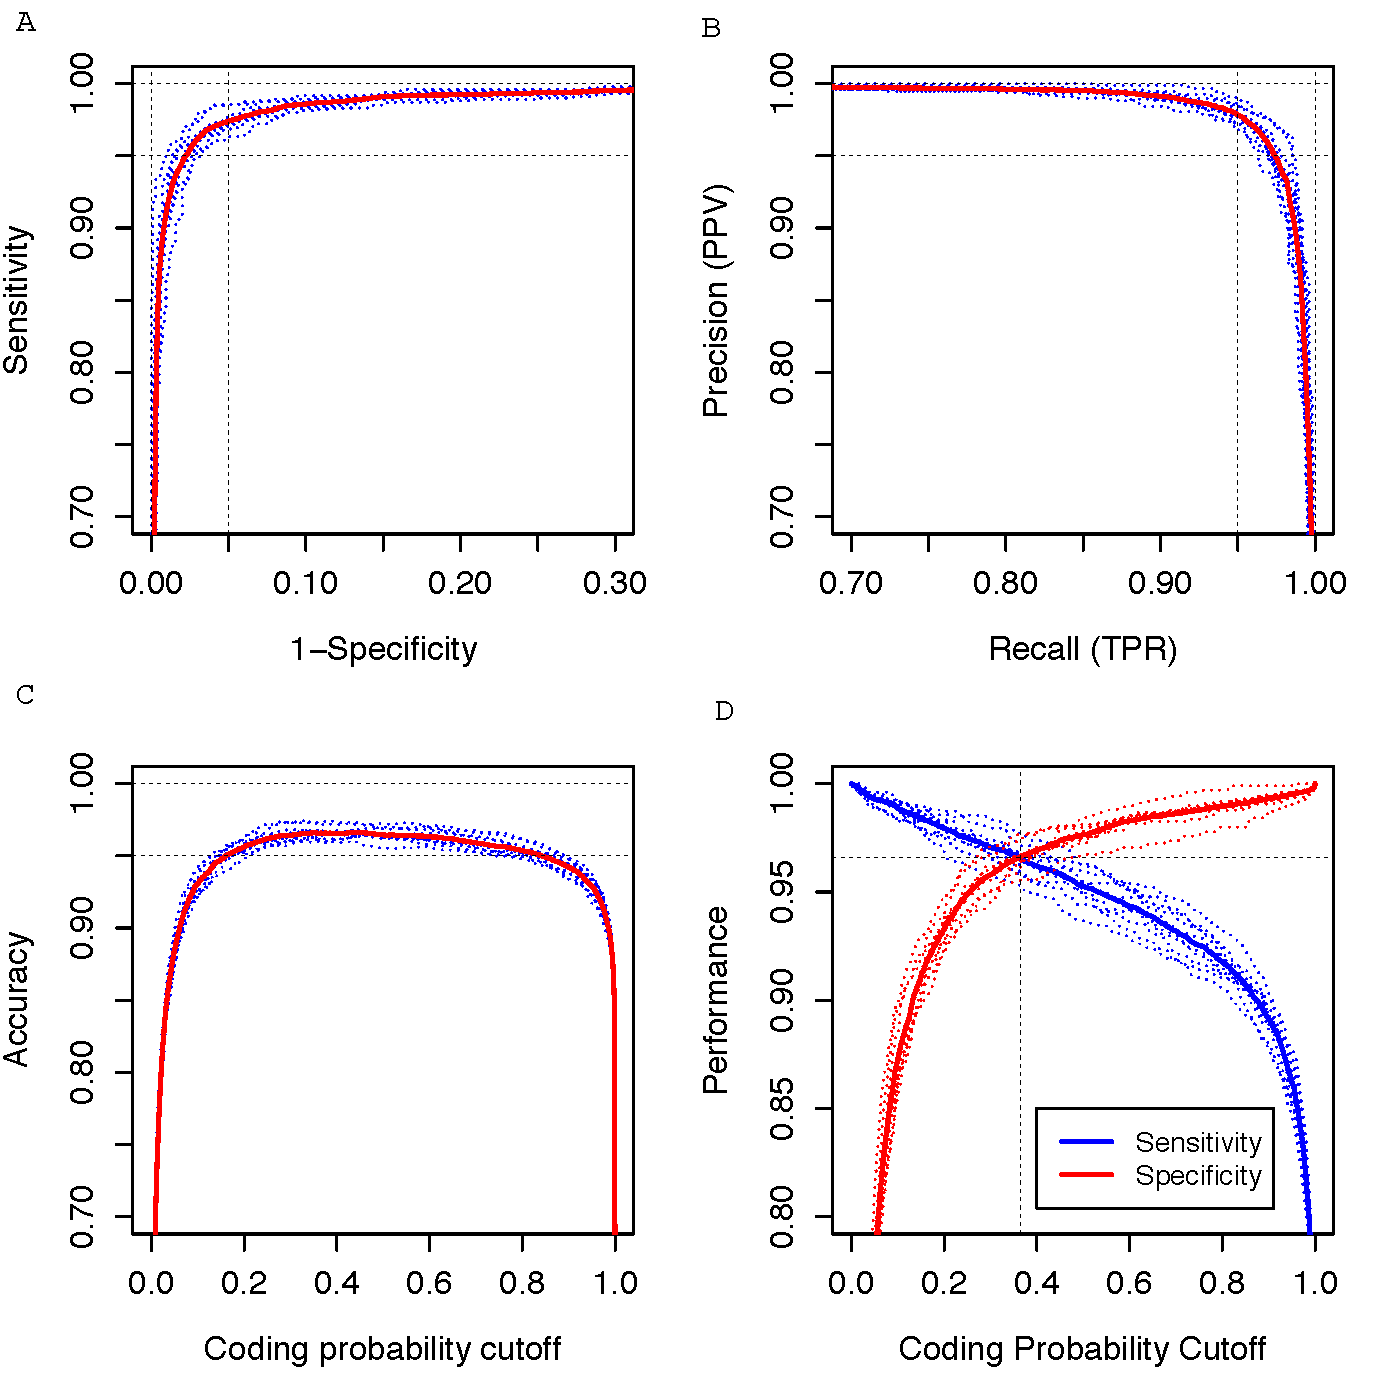
\includegraphics{CPAT_performance.png}}
\end{figure}


\chapter{Comparison}
\label{index:comparison}
To compare CPAT with CPC and PhyloCSF, we build an independent testing dataset that composed
of 4,000 high quality protein coding genes from Refseq annotation and 4,000 lincRNAs from
Human lincRNA catalog (Cabili et al., 2011). All 8000 genes were not included in the training
dataset of CPAT.
\begin{figure}[htbp]
\centering

\scalebox{1.000000}{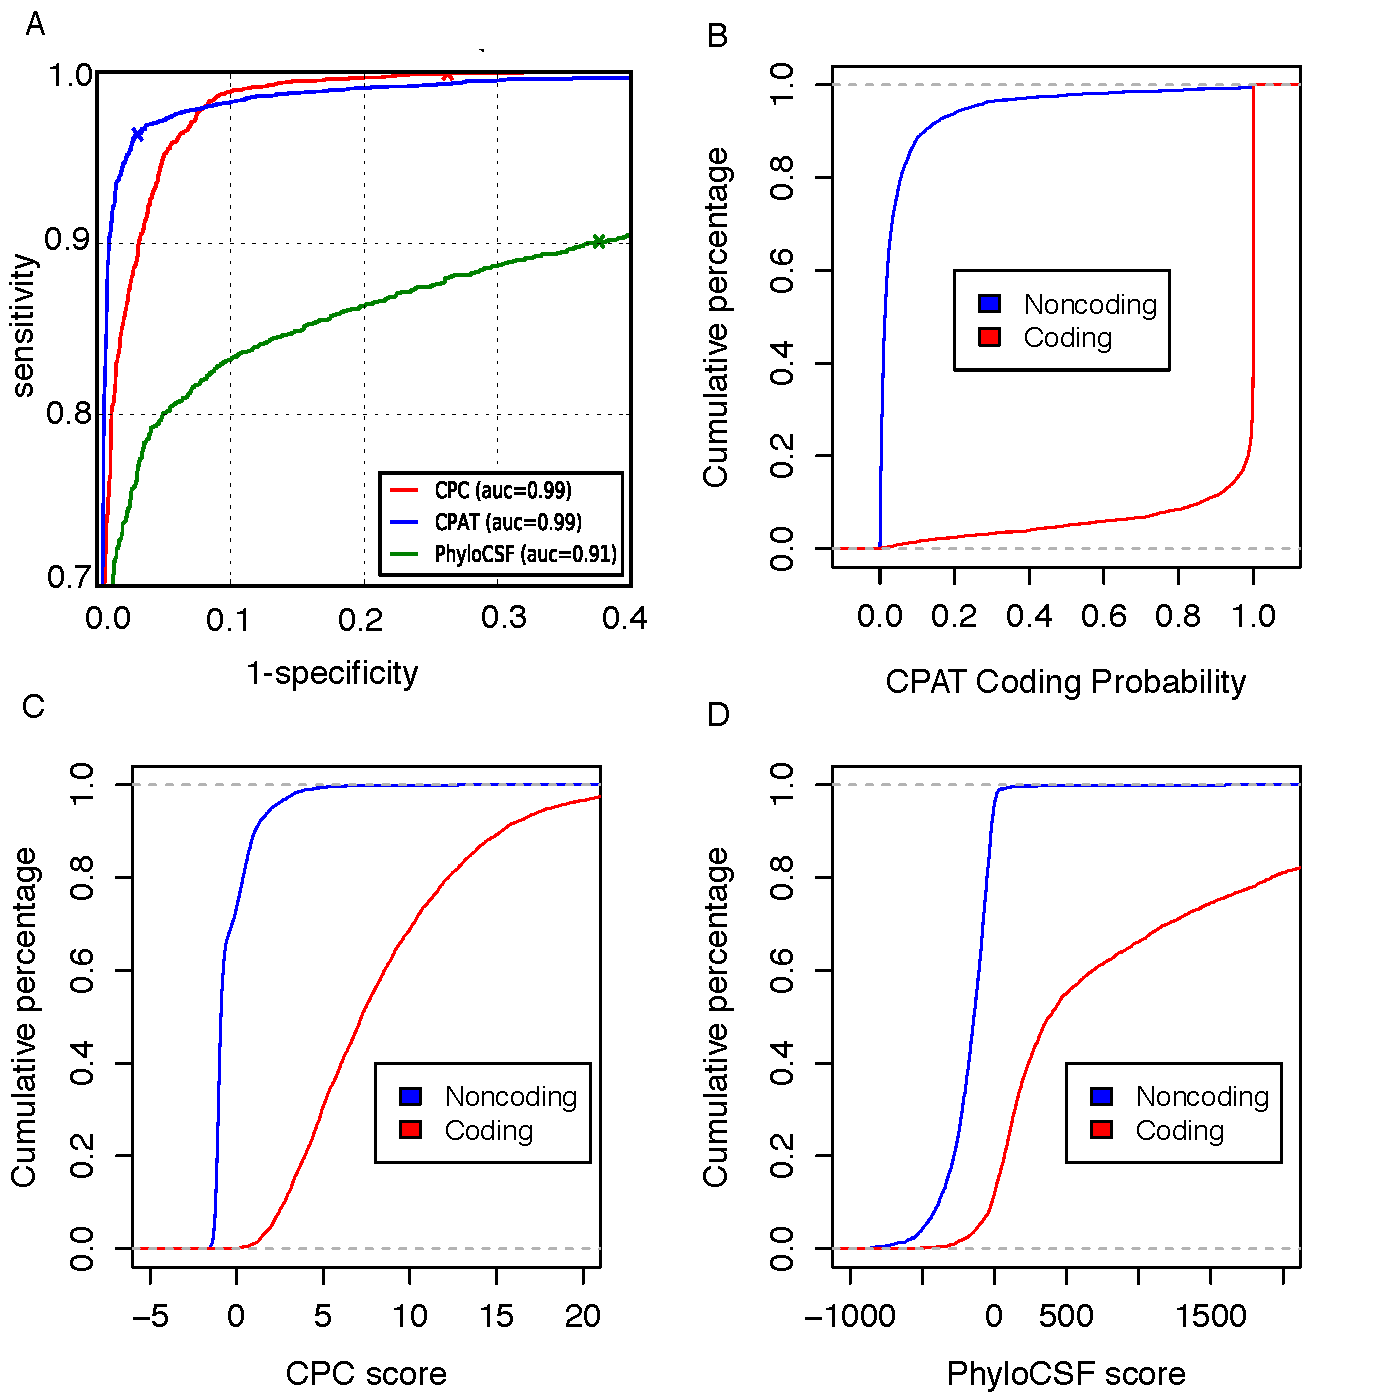
\includegraphics{Figure_4.png}}
\end{figure}
\begin{figure}[htbp]
\centering

\scalebox{1.000000}{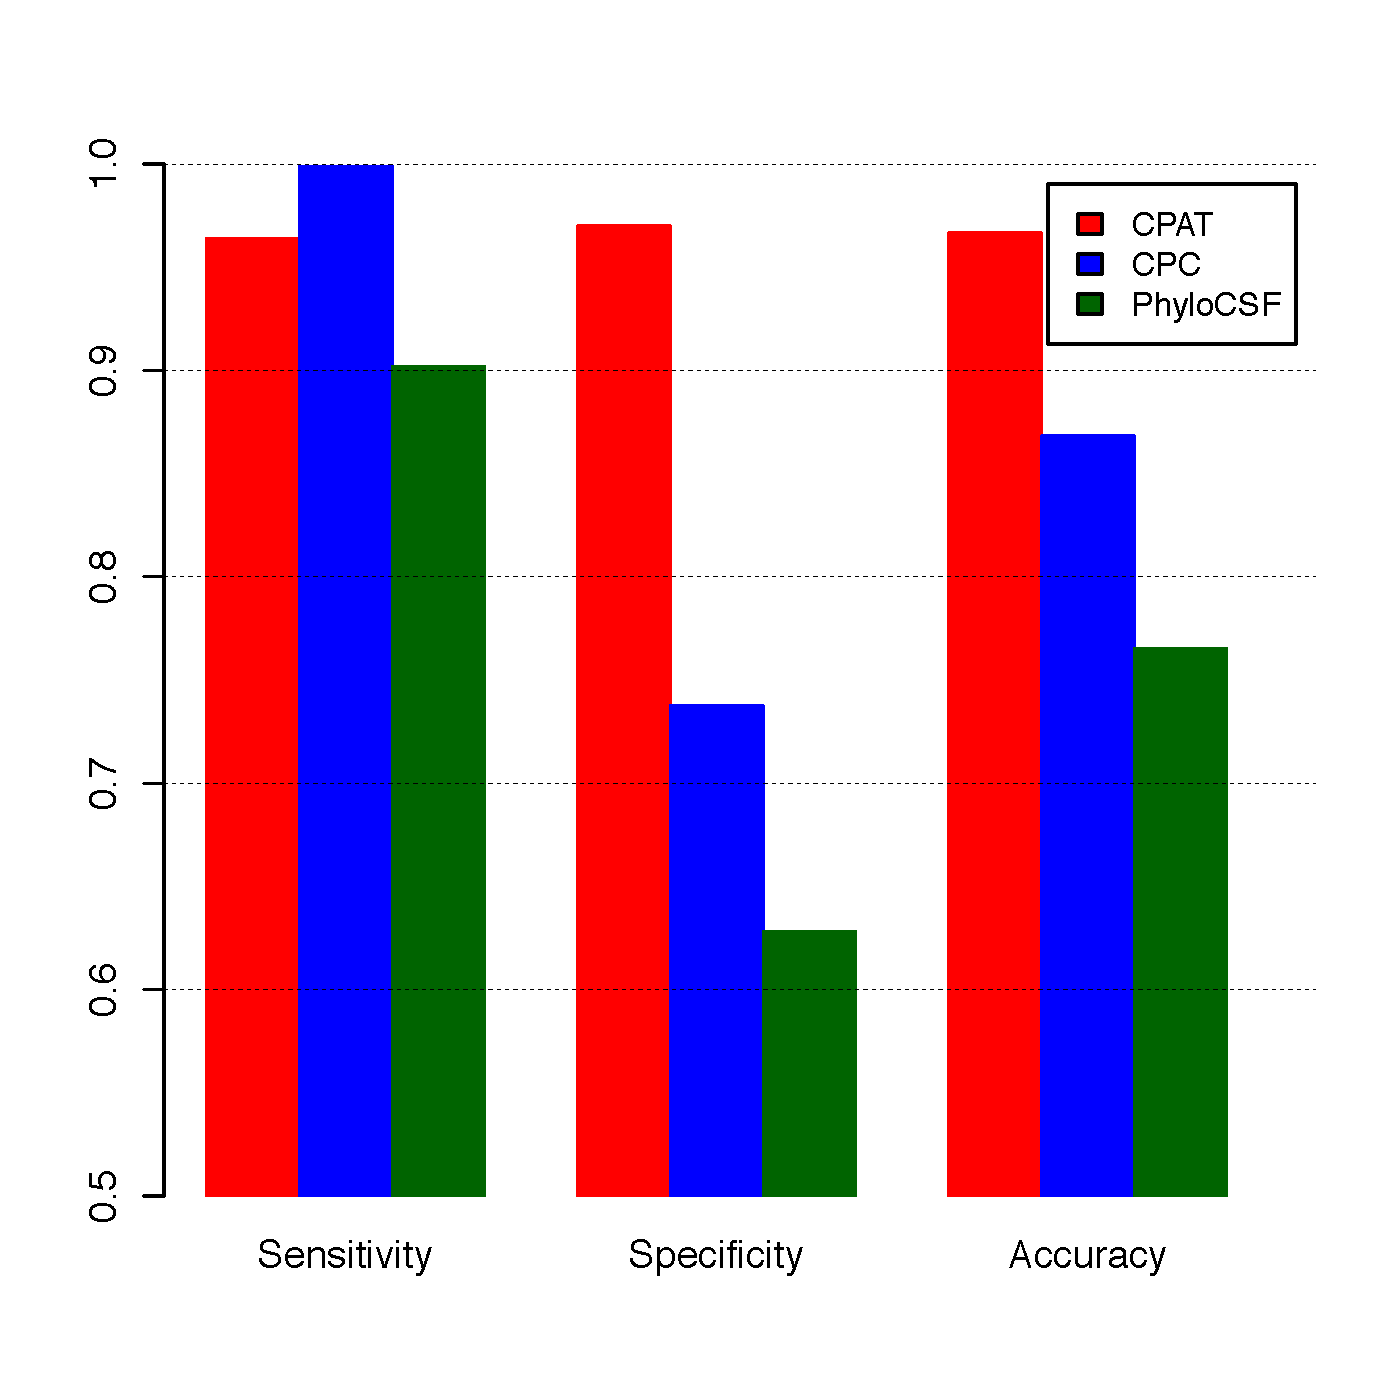
\includegraphics{Figure_S2.png}}
\end{figure}


\chapter{LICENSE}
\label{index:license}
CPAT is distributed under \href{http://www.gnu.org/copyleft/gpl.html}{GNU General Public License}

This program is free software; you can redistribute it and/or
modify it under the terms of the GNU General Public License as
published by the Free Software Foundation; either version 2 of the
License, or (at your option) any later version. This program is distributed in the hope that it will be useful,
but WITHOUT ANY WARRANTY; without even the implied warranty of
MERCHANTABILITY or FITNESS FOR A PARTICULAR PURPOSE.  See the GNU
General Public License for more details. You should have received a copy of the GNU General Public License
along with this program; if not, write to the Free Software
Foundation, Inc., 51 Franklin Street, Fifth Floor, Boston, MA
02110-1301 USA


\chapter{Contact}
\label{index:contact}\begin{itemize}
\item {} 
Liguo Wang: wang.liguo AT mayo.edu

\item {} 
Hyun Jung Park: hjpark AT bcm.edu

\end{itemize}



\renewcommand{\indexname}{Index}
\printindex
\end{document}
